%%%%% Physik Kompendium Nr.2 %%%%%
%% 05 -- Widerstände im Wechselstromkreis %%


Während es im Gleichstromkreis nur den Ohm'schen Widerstand gibt, betrachten wir im Wechselstromkreis drei Typen.

Zwei Arten, der kapazitive und der induktive Widerstand, generieren nur Phasenverschiebungen, die in Blindwiderstand resultieren.


\subsection{Ohm'sche Widerstände}		\label{subsec:OhmscherWiderstand}

Wenn in einem Wechselstromkreis nur ein Ohm'scher Widerstand verbaut ist, ist die Impedanz $Z$, also der Gesamtwiderstand des Kreises, gleich dem Wert dieses Widerstandes.

Das bedeutet, er verursacht keine Phasenverschiebung und kann wie ein Widerstand des Gleichstromkreises behandelt werden.


\subsection{Kapazitive Widerstände}		\label{subsec:KapazitiverWiderstand}

Der Kapazitive Widerstand geht von einem Kondensator aus. Da Kondensatoren keinen Durchfluss erlauben, ist ihr Widerstand im Gleichstromkreis unendlich. Im Wechselstromkreis verursacht er aber eine Phasenverschiebung des Stromes, welcher dann um 90\degree der Spannung vorauseilt.

Beim Wechselstrom schwingen die elektrischen Ladungen jedoch hin und her. Ein Kondensator im Wechselstromkreis wird also abwechselnd geladen und wieder entladen. Die Spannung zwischen den Kondensatorpolen baut sich während des Ladevorgangs auf und erreicht ihr Maximum dann, wenn der Kondensator vollständig aufgeladen und der Stromfluss zum Erliegen gekommen ist. Beim Entladevorgang sind die Verhältnisse umgekehrt: Die Stromstärke ist dann am größten, wenn der Kondensator vollständig entladen ist. \footnotemark

\footnotetext{Paragraph von: \url{http://files.sma.de/dl/10040/BLINDLEISTUNG-ADE094210.pdf}}

\glqq Der Strom eilt der Spannung voraus.\grqq

\vspace{11pt}

Dieser sogenannte \glqq Kapazitive Blindwiderstand\grqq{} ist antiproportional abhängig von der Kapazität des Kondensators und der Winkelgeschwindigkeit (siehe Sektion \ref{subsec:ErlaeuterungenGrundlegend} auf Seite \pageref{subsec:ErlaeuterungenGrundlegend}):

\begin{equation}	\label{eq:KapazitiverWiderstand}
	X_C = \frac{1}{\omega \cdot C}
\end{equation}


\subsection{Induktive Widerstände}		\label{subsec:InduktiverWiderstand}

Eine Spule leitet Gleichstrom wie ein normaler Draht. Nur beim Ein- und Ausschalten gibt es jeweils eine Zeitverzögerung im Stromfluss, die durch den Auf- und Abbau des Magnetfeldes verursacht wird. Unter Wechselstrombedingungen kommt es bei jedem Wechsel der Stromrichtung zu diesen Verzögerungen. Dies resultiert in einer Phasenverschiebung des Stromes um -90\degree .\footnotemark

\footnotetext{Paragraph von: \url{http://files.sma.de/dl/10040/BLINDLEISTUNG-ADE094210.pdf}}

\glqq Die Spannung eilt dem Strom voraus.\grqq

\vspace{11pt}

Der \glqq Induktive Widerstand\grqq{} ist abhängig von der Induktivität der Spule und der Winkelgeschwindigkeit (siehe Sektion \ref{subsec:ErlaeuterungenGrundlegend} auf Seite \pageref{subsec:ErlaeuterungenGrundlegend}):

\begin{equation}	\label{eq:InduktiverWiderstand}
	X_L = \omega \cdot  L
\end{equation}

%http://files.sma.de/dl/10040/BLINDLEISTUNG-ADE094210.pdf


\subsection{Auswirkungen von Blindwiderständen auf die Stromstärke} \label{subsec:AuswirkungenWiderstand}

Man kann die Gleichung für die Impedanz (Gleichung \ref{eq:Impedanz} auf Seite \pageref{eq:Impedanz}) nach $I$ umstellen, um sich zu verdeutlichen, dass eine erhöhte Impedanz eine niedrigere Stromstärke zur Folge hat, genau wie der Ohm'sche Widerstand im Wechselstromkreis:

\begin{equation}	\label{eq:ImitZ}
	I_{eff}=\frac{U_{eff}}{Z}
\end{equation}


\subsection{Frequenzabhängigkeit}	\label{subsec:Frequenzabhaengigkeit}

Die Größe der Blindwiderstände ist sowohl beim Kondensator als auch bei der Spule abhängig von der Frequenz des Wechselstromes (diese Steckt im $\omega$).

Der kapazitive Blindwiderstand ist antiproportional abhängig (Siehe Gleichung \ref{eq:KapazitiverWiderstand}) von der Frequenz, was bedeutet: \glqq Ein Kondensator erhöht die Impedanz, je niedriger die Frequenz ist.\grqq{} Man sagt auch \glqq High-Pass-Filter\grqq{} oder \glqq Low-Cut-Filter\grqq .

Der induktive Blindwiderstand ist proportional abhängig (Siehe Gleichung \ref{eq:InduktiverWiderstand}) von der Frequenz, was bedeutet: \glqq Eine Spule erhöht die Impedanz, je höher die Frequenz ist.\grqq{} Man sagt auch \glqq Low-Pass-Filter\grqq oder \glqq High-Cut-Filter\grqq .



\subsection{Zeigerdiagramm}	\label{subsec:WiderstaendeZeigerdiagram}

Die Impedanz (Sektion \ref{subsec:ErlaeuterungenWeitere} auf Seite \ref{subsec:ErlaeuterungenWeitere}) ist auch berechenbar, wenn der Ohm'sche Widerstand und der Blindwiderstand bekannt ist. Bevor Gesetze betrachtet werden, ist das Zeigerdiagramm eine gute Veranschaulichung.

Auf einem Zeigerdiagramm lässt sich die Relation von Blindwiderstand, Ohmschen Widerstand, Scheinwiderstand (Impedanz) und dem Phasenverschiebungswinkel (Siehe Sektion \ref{subsec:ErlaeuterungenWeitere} auf Seite \ref{subsec:ErlaeuterungenWeitere}) darstellen:

\begin{figure}[h!]
	\centering
	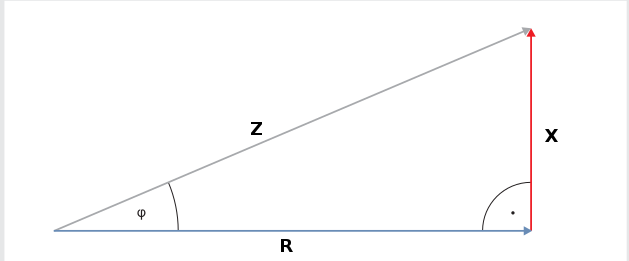
\includegraphics[width=0.9\textwidth]{Pictures/Zeigerdiagramm}
	\caption{Zeigerdiagramm mit Widerständen: Blau: Ohm'scher Widerstand, Rot: Blindwiderstand, Grau: Impedanz, $\varphi$: Phasenverschiebungswinkel}
	\footnotemark
\end{figure}

\footnotetext{Illustration von: \url{http://files.sma.de/dl/10040/BLINDLEISTUNG-ADE094210.pdf}}

\vspace{11pt}

Daraus folgt zum Beispiel, dass wenn nur eine ideale Spule (hat keinen zusätzlichen Ohm'schen Widerstand) oder ein Kondensator in einem Wechselstromkreis geschaltet sind, dies in einem Kurzschluss resultiert, da es keinen Ohm'schen Widerstand gibt und damit die Impedanz ebenfalls null ist.

Des Weiteren veranschaulicht das Diagramm den Zusammenhang von dem Verhältnis des Blindwiderstandes zum Ohm'schen Widerstand. Dieses Verhältnis ist nämlich immer gleich dem Tangenz des Winkels $\varphi$.

\paragraph{Anmerkung:}

Sollten in einem Schaltkreis beide Blindwiderstände (eine Spule und ein Kondensator) verbaut sein, muss für die Differenz angenommen werden, da die beiden Vektoren im Diagramm entgegengesetzt sein würden, da die Phasenverschiebung mit jeweils 90\degree{} in die entgegengesetzte Richtung ausgeführt wird. Das resultiert in einem Winkel von 180\degree :

\begin{equation}	\label{eq:BlindwiderstandSumme}
	X_{ges} = X_L - X_C = \omega \cdot L - \frac{1}{\omega \cdot C}
\end{equation}



\subsection{Gesetze}	\label{subsec:WiderstaendeGesetzte}

Nun ist auch die Betrachtung der Gesetze, angelehnt an diese Darstellungsform, deutlich einfacher.


Für die Impedanz können nun, zusätzlich zu Gleichung \ref{eq:Impedanz} auf Seite \pageref{eq:Impedanz}, noch andere Betrachtungen gefunden werden: \\ In Abhängigkeit von $X$ und $R$:

\begin{equation}	\label{eq:ImepdanzXR}
	Z = \sqrt{X^2 + R^2}
\end{equation}


\hspace{-6mm}In Abhängigkeit von $X$ und $\varphi$:

\begin{equation}	\label{eq:ImepdanzXphi}
	Z = \frac{X}{\sin\varphi}
\end{equation}


\hspace{-6mm}In Abhängigkeit von $R$ und $\varphi$:

\begin{equation}	\label{eq:ImepdanzRphi}
	Z = \frac{R}{\cos\varphi}
\end{equation}









